% DeltaCache Inference Flow - TikZ Figure
% Shows the request processing pipeline
% For IJCNN 2025 Paper

\documentclass[tikz,border=5pt]{standalone}
\usepackage{tikz}
\usetikzlibrary{shapes.geometric, arrows.meta, positioning, fit, backgrounds, calc, decorations.pathreplacing, shadows.blur}

% Color scheme
\definecolor{primaryblue}{RGB}{41, 98, 255}
\definecolor{secondaryblue}{RGB}{66, 133, 244}
\definecolor{lightblue}{RGB}{232, 240, 254}
\definecolor{accentorange}{RGB}{255, 152, 0}
\definecolor{successgreen}{RGB}{52, 168, 83}
\definecolor{lightgreen}{RGB}{232, 245, 233}
\definecolor{warningred}{RGB}{234, 67, 53}
\definecolor{lightred}{RGB}{253, 237, 237}
\definecolor{neutralgray}{RGB}{95, 99, 104}
\definecolor{lightgray}{RGB}{248, 249, 250}
\definecolor{darktext}{RGB}{32, 33, 36}

\begin{document}
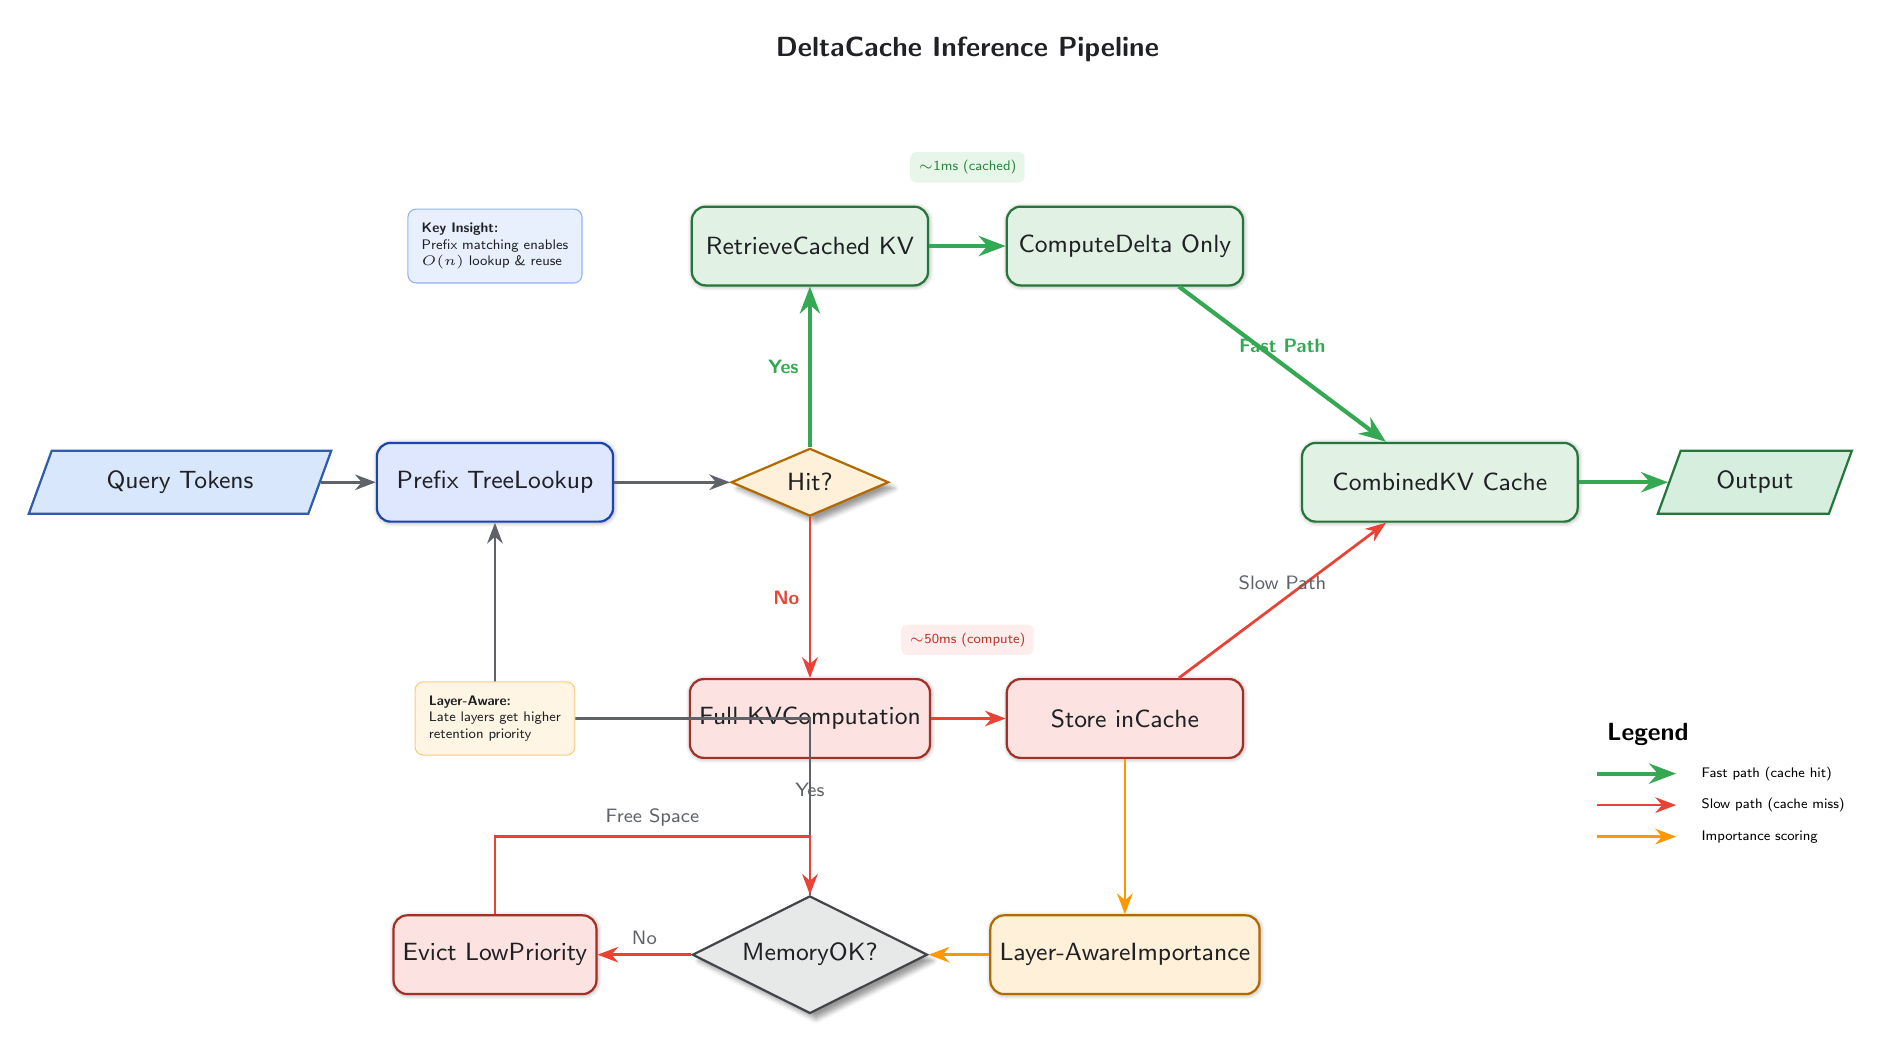
\begin{tikzpicture}[
    % Node styles
    process/.style={
        rectangle,
        rounded corners=5pt,
        minimum width=2.5cm,
        minimum height=1cm,
        draw=#1!70!black,
        fill=#1!15,
        line width=0.8pt,
        font=\small\sffamily,
        text=darktext,
        blur shadow={shadow blur steps=5, shadow xshift=0.3pt, shadow yshift=-0.3pt}
    },
    decision/.style={
        diamond,
        aspect=2,
        minimum width=2cm,
        draw=#1!70!black,
        fill=#1!15,
        line width=0.8pt,
        font=\small\sffamily,
        text=darktext,
        blur shadow={shadow blur steps=5}
    },
    io/.style={
        trapezium,
        trapezium left angle=70,
        trapezium right angle=110,
        minimum width=2cm,
        minimum height=0.8cm,
        draw=#1!70!black,
        fill=#1!20,
        line width=0.8pt,
        font=\small\sffamily,
        text=darktext
    },
    arrow/.style={
        ->,
        >=Stealth,
        line width=1pt,
        #1
    },
    label/.style={
        font=\scriptsize\sffamily,
        text=neutralgray
    },
    speedlabel/.style={
        font=\scriptsize\sffamily\bfseries,
        text=#1
    }
]

% ============================================
% Input
% ============================================
\node[io=secondaryblue] (input) at (0, 0) {Query Tokens};

% ============================================
% Prefix Tree Lookup
% ============================================
\node[process=primaryblue, minimum width=3cm] (lookup) at (4, 0) {Prefix Tree\\Lookup};

% ============================================
% Decision: Cache Hit?
% ============================================
\node[decision=accentorange] (decision) at (8, 0) {Hit?};

% ============================================
% Cache Hit Path (Fast)
% ============================================
\node[process=successgreen, minimum width=3cm] (retrieve) at (8, 3) {Retrieve\\Cached KV};
\node[process=successgreen, minimum width=3cm] (delta) at (12, 3) {Compute\\Delta Only};

% ============================================
% Cache Miss Path (Slow)
% ============================================
\node[process=warningred, minimum width=3cm] (compute) at (8, -3) {Full KV\\Computation};
\node[process=warningred, minimum width=3cm] (store) at (12, -3) {Store in\\Cache};

% ============================================
% Importance Scoring
% ============================================
\node[process=accentorange, minimum width=3cm] (importance) at (12, -6) {Layer-Aware\\Importance};

% ============================================
% Memory Check
% ============================================
\node[decision=neutralgray, minimum width=1.5cm] (memcheck) at (8, -6) {Memory\\OK?};

% ============================================
% Eviction
% ============================================
\node[process=warningred, minimum width=2.5cm] (evict) at (4, -6) {Evict Low\\Priority};

% ============================================
% Output
% ============================================
\node[process=successgreen, minimum width=3.5cm] (output) at (16, 0) {Combined\\KV Cache};
\node[io=successgreen] (result) at (20, 0) {Output};

% ============================================
% Arrows
% ============================================

% Input to lookup
\draw[arrow=neutralgray] (input) -- (lookup);

% Lookup to decision
\draw[arrow=neutralgray] (lookup) -- (decision);

% Cache hit path
\draw[arrow=successgreen, line width=1.5pt] (decision) -- node[left, speedlabel=successgreen] {Yes} (retrieve);
\draw[arrow=successgreen, line width=1.5pt] (retrieve) -- (delta);
\draw[arrow=successgreen, line width=1.5pt] (delta) -- node[above, speedlabel=successgreen] {Fast Path} (output);

% Cache miss path
\draw[arrow=warningred] (decision) -- node[left, speedlabel=warningred] {No} (compute);
\draw[arrow=warningred] (compute) -- (store);
\draw[arrow=warningred] (store) -- node[above, label] {Slow Path} (output);

% Store to importance
\draw[arrow=accentorange] (store) -- (importance);

% Importance to memcheck
\draw[arrow=accentorange] (importance) -- (memcheck);

% Memcheck paths
\draw[arrow=neutralgray] (memcheck) -- node[above, label] {Yes} ++(0, 3) -| (lookup);
\draw[arrow=warningred] (memcheck) -- node[above, label] {No} (evict);
\draw[arrow=warningred] (evict) -- ++(0, 1.5) -| node[above, label, pos=0.25] {Free Space} (memcheck);

% Output to result
\draw[arrow=successgreen, line width=1.5pt] (output) -- (result);

% ============================================
% Speed annotations
% ============================================
\node[fill=lightgreen, rounded corners=2pt, font=\tiny\sffamily, text=successgreen!80!black, inner sep=3pt] at (10, 4) {$\sim$1ms (cached)};
\node[fill=lightred, rounded corners=2pt, font=\tiny\sffamily, text=warningred!80!black, inner sep=3pt] at (10, -2) {$\sim$50ms (compute)};

% ============================================
% Legend box
% ============================================
\begin{scope}[shift={(18, -4)}]
    \node[font=\small\sffamily\bfseries, anchor=west] at (0, 0.8) {Legend};
    \draw[arrow=successgreen, line width=1.5pt] (0, 0.3) -- ++(1, 0);
    \node[font=\tiny\sffamily, anchor=west] at (1.2, 0.3) {Fast path (cache hit)};
    \draw[arrow=warningred] (0, -0.1) -- ++(1, 0);
    \node[font=\tiny\sffamily, anchor=west] at (1.2, -0.1) {Slow path (cache miss)};
    \draw[arrow=accentorange] (0, -0.5) -- ++(1, 0);
    \node[font=\tiny\sffamily, anchor=west] at (1.2, -0.5) {Importance scoring};
\end{scope}

% ============================================
% Title
% ============================================
\node[font=\normalsize\sffamily\bfseries, text=darktext] at (10, 5.5) {\textsc{DeltaCache} Inference Pipeline};

% ============================================
% Key insight box
% ============================================
\node[draw=primaryblue!50, fill=lightblue, rounded corners=3pt,
      font=\tiny\sffamily, text=darktext, align=left, inner sep=5pt]
      at (4, 3) {
    \textbf{Key Insight:}\\
    Prefix matching enables\\
    $O(n)$ lookup \& reuse
};

\node[draw=accentorange!50, fill=accentorange!10, rounded corners=3pt,
      font=\tiny\sffamily, text=darktext, align=left, inner sep=5pt]
      at (4, -3) {
    \textbf{Layer-Aware:}\\
    Late layers get higher\\
    retention priority
};

\end{tikzpicture}
\end{document}
